\chapter{Minimal Enclosing Ellipsoid of Ellipsoids}\label{chapter:meee}

\section{Uses of MEEE}

\PARstart{T}{he idea} of approximating complicated objects using simpler ones is widely used in computational geometry
and computer graphics. A common approach is to replace a complicated object by a simpler model covering it, such as a
minimum volume box or a sphere. More recently, ellipsoidal models have been proposed in the literature as they usually
provide better approximations than bounding boxes or spheres~\cite{yildirim06,sturm03,shiang00,ju01}. The use of simpler
objects inevitably leads to faster processing times for more responsive applications, ideally with minimal---though not
insignificant---loss of detail resolution. Recently new algorithms have been developed for the calculation of a minimal
enclosing ellipsoid; specifically, such an ellipsoid bounding the convex hull of a set of ellipsoids, also known as a
L\"owner ellipsoid, or L\"owner-John ellipsoid~\cite{yildirim06}.


% MAXDET 
\section{Solving with MAXDET}

The maxdet-problem is a convex optimization problem, minimizing the objective function
\begin{equation}\label{eqn:maxdetobj}
    c^T\v{x} + \log \det G(\v{x})^{-1}
\end{equation}
subject to
\begin{align}
     G(\v{x}) &>     0,\qquad\text{and}\nonumber\\
     F(\v{x}) &\geq  0,\label{eqn:maxdetcons}
\end{align}
where the optimization variable is the vector $\v{x}\in\Re^m$. The Functions 
$G:\Re^m\rightarrow\Re^{\left|\v{x}\right|}$ and $F:\Re^m\rightarrow\Re^{n\times n}$ are affine:
\begin{align}
    G(\v{x}) &= G_0 + \v{x}_1G_1 + \dots + \v{x}_mG_m\nonumber\\
    F(\v{x}) &= F_0 + \v{x}_1F_1 + \dots + \v{x}_mF_m\label{eqn:maxdet},
\end{align} 
where $G_i=G_i^T$ and $F_i=F_i^T$. The objective function is convex on $\{x|G(x)>0\}$ and the constraint set is
convex~\cite{vandenberghe96}.

A wide class of computational geometry problems can be formulated at maxdet-problems. The formulation of interest is
that of a minimal volume ellipsoid $\varepsilon_0$ containing $n$ given ellipsoids $\varepsilon_1\dots\varepsilon_n$. The
given ellipsoids are described as sublevel sets of convex quadratic functions:~\cite{vandenberghe96,boyd04}
\begin{equation}\label{eqn:ellipse}
    \varepsilon_i = \{ x | x^TA_ix + 2b_i^Tx + c_i \leq 0 \},\qquad i=0,\dots,n.
\end{equation}
The solution can be found by, in the variables $A_0 = A_0^T$, $b_0$, and
$n$ scalar variables $\tau_i$, minimizing:~\cite{vandenberghe96}
\begin{equation}\label{eqn:maxdetfun}
    \log\det A_0^{-1}
\end{equation}
subject to
\begin{equation}\label{eqn:maxdetconstraints}
    \begin{array}{l}
    A_0 = A_0^T > 0 ,\\
    \tau_1 \geq 0,\dots,\tau_n\geq 0 ,\qquad\text{and}\\
    \left[ \begin{array}{ccc}
        A_0   & b_0 &  0     \\
        b_0^T & -1  & b_0^T  \\
        0     & b_0 & -A_0
    \end{array} \right]
    -\tau_i
    \left[ \begin{array}{ccc}
        A_i   & b_i & 0 \\
        b_i^T & c_i & 0 \\
        0     &   0 & 0 
    \end{array} \right]
    \leq 0,\qquad i=1,\dots,n.
    \end{array}
\end{equation}
Here, $c_0$ is given by~\cite{boyd94}
\begin{equation}
    c_0=b_0^TA_0^{-1}b_0-1\\
\end{equation}
and the final ellipsoid is
\begin{equation}
    \varepsilon_0=\{x|x^TA_0x+2b_0^Tx+c_0\leq 0\},
\end{equation}
which defines the ellipsoid of least volume containing $\varepsilon_1,\dots,\varepsilon_n$. The formulation for the MEEE
constraints given in equation \ref{eqn:maxdetconstraints} as a maxdet-problem, as in equation \ref{eqn:maxdet}, 
is~\cite{vandenberghe96}.
\begin{align}
    G(\v{x}) &= I_{n\times n}\nonumber\\
    F(\v{x}) &= \left[\begin{array}{cccc}
        A_0 &   &  &  \\
            & \left[ \begin{array}{ccc}
                \tau_i A_i - A_0   & \tau_i b_i - b_0 &  0     \\
                \tau_i b_i^T - b_0^T & \tau_i c_i -1  & -b_0^T  \\
                0     & -b_0 & A_0
                \end{array}\right]  &  &  \\
            &   & \ddots & \\
            &   &  & 
                \left[ \begin{array}{ccc}
                \tau_1 &  &  \\
                       & \ddots & \\
                       &       & \tau_n
            \end{array}\right]
    \end{array}\right]
\end{align}
The variables $A_0$ and $b_0$, and $\tau_1\dots \tau_n$, are solved in-place during the minimization process.
\begin{figure}[tbp]
    \centering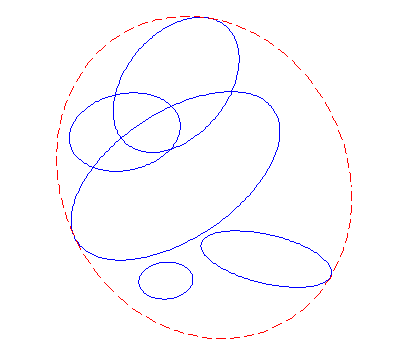
\includegraphics[width=0.6\textwidth]{figures/ellipse01.png}
    \caption{\it An example of a minimally enclosing L\"owner 2D ellipsoid containing five ellipsoids,
        from~\cite{boyd04}. Comparing this plot with figure \ref{fig:cu2d-gen-batch} will illustrate the superficial
        similarities between GCU and MEEE. }
    \label{fig:ellipse}
\end{figure}

Other convex optimization tools may be easily used with the objective function and constraints given in equations
\ref{eqn:maxdetfun} and \ref{eqn:maxdetconstraints} as well~\cite{boyd04}.


% CONTAINMENT
\section{Testing for Ellipsoid Containment}\label{section:containment}

In the development of any algorithm which finds a minimally enclosing object, it is necessary to also develop a test to
compare this theoretically enclosing result with its enclosed set. For the MEEE problem, the goal is to test whether one
ellipsoid properly contains another, i.e. the properly contained ellipsoid does not have any points which fall outside
the bounding perimeter of the containing ellipsoid~\cite{yildirim06}.

This analysis follows the test for ellipse intersection presented in~\cite{eberly00}. Consider an $n$--dimensional
ellipsoid $\varepsilon_0$ given by the curve,
\begin{equation}
    Q_0 = x^TA_0x + 2b_0^Tx + c_0,
\end{equation}
which should contain the $n$--dimensional ellipsoid $\varepsilon_1$ given by the curve,
\begin{equation}
    Q_1 = x^TA_1x + 2b_1^Tx + c_1.
\end{equation}
All level curves defined by $Q_0(x)=\lambda$ are ellipsoids, except for the minimum negative value of $\lambda$ for
which the equation defined a single point, the center of every level curve ellipsoid. The ellipsoid defined by
$Q_1(x)=0$ generally intersects many level curves of $Q_0$. By finding the minimum level value $\lambda_{min}$ and the
maximum level value $\lambda_{max}$ of $Q_0$ attained by any $x$ on the curve $Q_1$, it is possible to determine the
spatial relationship between $\varepsilon_0$ and $\varepsilon_1$. If $\lambda_{max}\leq 0$, then only a level curve
$Q_0(x)\leq 0$ will intersect $Q_1(x)=0$, and $\varepsilon_0$ must properly contain $\varepsilon_1$.

This can be formulated as a constrained minimization that can be solved by the method of Lagrange multipliers: Minimize
$Q_0(x)$ subject to the constraint that $Q_1(x)=0$. Define $F(x,t)=Q_0(x)+tQ_1(x)$. Differentiating yields $\nabla
F=\nabla Q_0+t\nabla Q_1$, where the gradient indicated derivative in $x$. Since $\partial{F}/\partial{t}=Q_1$, setting the
$t$-derivative equal to zero reproduces the constraint $Q_1=0$. Setting the $x$-derivative equal to zero yields $\nabla
Q_0+t\nabla Q_1=0$ for some $t$. Geometrically, this means the gradients are parallel.

Note that $\nabla Q_i=2A_ix+2b_i$, so
\begin{equation}
    0 = \nabla Q_0 + t\nabla Q_1 = 2(A_0+tA_1)x+2(b_0+tb_1).
\end{equation}
Solving for $x$ yields
\begin{equation}\label{eqn:solvex}
    x = -(A_0+tA_1)^{-1}(b_0+tb_1)=\frac{1}{\delta(t)}Y(t),
\end{equation}
where $\delta(t)$ is the determinant of $(A_0+tA_1)$, a polynomial in $t$ of degree $n$, and $Y(t)$ has components in
$t$ of degree $n$ as well. Replacing this in $Q_1(x)=0$ yields
\begin{equation}\label{eqn:poly}
    P(t) = Y(t)^TA_1Y(t)+\delta(t)b_1^TY(t)+\delta(t)^2c_1=0,
\end{equation}
a degree $2n$ polynomial in $t$. The roots of $P(t)$ in equation \ref{eqn:poly} can be applied to equation
\ref{eqn:solvex} to find the critical values for $x$ of $Q_1$. The minimum and maximum values of the evaluation of
$Q_0(x)$ at the roots of $P(t)$ are respectively $\lambda_{min}$ and $\lambda_{max}$, the minimum and maximum level
curves which intersect $Q_1$. 

As stated previously, if $\lambda_{max}\leq 0$, then $\varepsilon_0$ properly contains $\varepsilon_1$.


% TRANSFORM
\section{Relating to Generalized Covariance Union}

Before any MEEE results can be compared to GCU, it is necessary to define a set of transforms between the ellipsoid and
statistical measurement domains.  Since this thesis interprets all estimates (means and covariances) as unweighted
Gaussian PDFs, i.e.
\begin{equation}
    (\v{m}_i,\m{M}_i) := \gaussN{\v{m}_i,\m{M}_i},
\end{equation}
each estimate is uniquely transformable to and from the ellipsoid domain, given in equation \ref{eqn:ellipse},
by representing each as only the 1-$\sigma$ contour ellipsoid on its Gaussian surface. The
forward transformation into ellipse notation is~\cite{boyd04}
\begin{align}
\label{eqn:cu2e}
\mathbb{T}(\v{m}_i,\m{M}_i) &:= \left\{
    \begin{aligned}
        A_i &= \m{M}_i^{-1}\\
        b_i &= -\m{M}_i^{-1}\v{m}_i\\
        c_i &= \v{m}_i^T\m{M}_i^{-1}\v{m}_i-1,
    \end{aligned}
    \right.
\intertext{and the backward transformation is}
\label{eqn:e2cu}
\mathbb{T}^{-1}(A_i,b_i,c_i) &:= \left\{
    \begin{aligned}
        \m{M}_i &= A_i^{-1}\\
        \m{m}_i &= -A_i^{-1}b_i.
    \end{aligned}
    \right.
\end{align}
The ellipsoid described by $(A_i,b_i,c_i)$ is centered at $\v{m}_i$, with a radial distance of $\m{M}_i^{\frac{1}{2}}$.
By interpreting a given Gaussian PDF as an ellipsoid, or a given ellipsoid as the 1-$\sigma$ contour which defines a
Gaussian PDF, it is possible to directly compare the results of GCU and MEEE.







